%% =====================================================================
%% Springer Nature LaTeX wrapper for journal: Automated Software
%% Engineering (ASE-J). Target submission template.
%%
%% REQUIRES the Springer Nature template package (sn-jnl.cls + .bst),
%% which is NOT bundled with this repo. Obtain it from:
%%   https://www.springernature.com/gp/authors/campaigns/latex-author-support
%%   or the Overleaf template "Springer Nature LaTeX Template".
%% Drop sn-jnl.cls and the sn-*.bst files next to this file, then build:
%%   pdflatex main_snj  &&  bibtex main_snj  &&  pdflatex main_snj x2
%%
%% This wrapper reuses the SAME section files as the IEEE version
%% (01_intro..06_conclusion) so content stays single-source. Only the
%% title block, abstract, keywords, and bibliography differ here.
%% See REFORMAT_ASE-J.md for the conversion checklist.
%% =====================================================================

% Math & Physical Sciences reference style, numbered (conventional for ASE-J).
\documentclass[pdflatex,sn-mathphys-num]{sn-jnl}

\usepackage{graphicx}
\usepackage{booktabs}
\usepackage{amsmath,amssymb,amsfonts}
\usepackage{multirow}
\usepackage{url}

\begin{document}

\title[Multi-Task Evaluation of LLMs on Software Engineering Tasks]{%
Comprehensive Evaluation of Large Language Models on Software Engineering
Tasks: A Multi-Task Benchmark}

%% Both authors are at UBHINUS (Malang). Optional refinements before submit:
%%  - add \orgdiv{Department/Faculty} if required by the journal
%%  - add \orcid{...} per author (recommended by Springer)
\author[1]{\fnm{Go Frendi} \sur{Gunawan}}\email{gofrendiasgard@gmail.com}
\author*[1]{\fnm{Mukhlis} \sur{Amien}}\email{amien@ubhinus.ac.id}

\affil[1]{\orgname{Universitas Bhinneka Nusantara (UBHINUS)},
  \city{Malang}, \country{Indonesia}}

\abstract{Large Language Models (LLMs) have demonstrated remarkable
capabilities in software engineering, yet comprehensive benchmarks covering
diverse SE activities remain limited. We present a multi-task evaluation of 11
state-of-the-art LLMs across five representative software engineering tasks:
bug fixing, feature development, code refactoring, technical copywriting, and
research synthesis. Our automated verification framework measures both output
quality and completion efficiency. Key findings reveal that (1) models
achieving identical perfect scores exhibit 22$\times$ variation in completion
time, 49$\times$ variation in tool efficiency, and 53$\times$ variation in
estimated cost; (2) tool usage frequency shows no correlation with success
($r=0.077$, $p=0.575$)---one model used 917 tool calls while another solved
the same task with 3 calls; (3) we identify two distinct inefficiency
patterns: \textit{loop inefficiency} (repetitive tool sequences) and
\textit{inference inefficiency} (slow token generation); and (4) coding tasks
achieve 100\% success while research tasks present greater challenges
(90.9\%). These results provide evidence-based guidance for practitioners
selecting LLMs based on task requirements, speed constraints, and budget
considerations. We release all experimental data, verification scripts, and
analysis code for full reproducibility.}

\keywords{Large Language Models, Software Engineering, Benchmark,
Code Generation, Evaluation, Efficiency}

\maketitle

%% Section content is shared with the IEEE build (main.tex).
\section{Introduction}
\label{sec:intro}

Large Language Models (LLMs) have demonstrated remarkable capabilities in software engineering tasks, from code generation and bug fixing to documentation and architectural design \cite{chen2021evaluating, jimenez2023swe}. As these models become increasingly integrated into development workflows, practitioners face a critical question: which model should they choose for specific tasks?

\subsection{Motivation}

The landscape of LLMs for code has expanded rapidly. OpenAI's GPT-4 and its successors have set benchmarks in coding proficiency \cite{openai2024gpt4}. Google's Gemini series offers competitive performance with different architectural approaches \cite{gemini2024}. Open-weight alternatives like Deepseek, GLM, and Qwen provide options for organizations with data privacy or cost constraints \cite{deepseek2024, glm2024, qwen2024}.

However, practitioners face several challenges when selecting models:

\begin{enumerate}
    \item \textbf{Fragmented benchmarks:} Existing evaluations focus on isolated capabilities (e.g., function-level code generation \cite{chen2021evaluating} or bug fixing \cite{jimenez2023swe}) rather than comprehensive software engineering workflows.
    
    \item \textbf{Task-specific studies:} Most evaluations test single task types, leaving unclear how models generalize across diverse activities like refactoring, documentation, and research.
    
    \item \textbf{Efficiency metrics:} Prior work often emphasizes accuracy alone, ignoring practical constraints like completion time and API costs.
    
    \item \textbf{Tool integration:} Modern LLMs operate through agent frameworks with tool use, yet few evaluations measure tool efficiency alongside output quality.
\end{enumerate}

\subsection{Research Questions}

This study addresses these gaps through systematic evaluation of 11 state-of-the-art LLMs across five representative software engineering tasks. We investigate:

\begin{description}
    \item[RQ1] How do current LLMs rank in overall performance across diverse software engineering tasks?
    \item[RQ2] Which models excel at specific task types (coding, writing, research)?
    \item[RQ3] What is the relationship between tool usage frequency and task success?
    \item[RQ4] How do completion time and accuracy correlate across models?
    \item[RQ5] What cost-performance tradeoffs exist across model tiers?
\end{description}

\subsection{Contributions}

Our work makes the following contributions:

\begin{enumerate}
    \item \textbf{Multi-task benchmark:} We present a comprehensive evaluation covering bug fixing, feature development, refactoring, technical writing, and research synthesis with automated verification.

    \item \textbf{Broad model comparison:} We evaluate 11 models from 4 provider categories (OpenAI, Google, Deepseek, Open-weight), enabling cross-provider analysis.

    \item \textbf{Efficiency analysis:} We introduce efficiency metrics (Tool Efficiency Ratio, Time Efficiency Ratio, Cost Estimation) revealing 22--53$\times$ variance among models achieving identical scores.

    \item \textbf{Inefficiency taxonomy:} We identify and categorize two distinct inefficiency patterns (loop vs inference), providing actionable insights for framework optimization.

    \item \textbf{Tool usage insights:} We analyze the relationship between tool invocation patterns and success, finding that more tools do not guarantee better results---917 vs 3 tool calls for identical outcomes.

    \item \textbf{Public dataset:} We release all experimental data, verification scripts, and results to enable reproducibility and future research \cite{our_dataset}.
\end{enumerate}

\subsection{Key Findings}

Our analysis reveals several surprising findings:

\begin{itemize}
    \item Four models (GPT-5.1, Gemini-3 Pro, Deepseek-Chat, GLM-4.7) achieved perfect scores, but exhibited dramatic efficiency variance: \textbf{22$\times$} in completion time (33s vs 732s), \textbf{49$\times$} in tool calls (3.8 vs 188 avg), and \textbf{53$\times$} in estimated cost.

    \item No correlation exists between tool usage count and success (Pearson $r=0.077$, $p=0.575$). GPT-5.1 solved bug-fix in 18.8s with 3 tools; Gemini-3 Flash took 625s with 917 tools---achieving identical EXCELLENT scores.

    \item We identify two distinct inefficiency patterns: (a) \textit{loop inefficiency}, where agents repeat tool sequences without recognizing failure, and (b) \textit{inference inefficiency}, where models generate correct solutions slowly.

    \item Research tasks were most challenging (90.9\% success), while coding tasks achieved 100\% success across all models.

    \item OpenAI models were consistently fastest (avg 54s) without sacrificing quality (9.33 avg score), offering the best speed-quality tradeoff.
\end{itemize}

\subsection{Paper Organization}

The remainder of this paper is organized as follows:
Section~\ref{sec:related} reviews related work in LLM evaluation.
Section~\ref{sec:methodology} describes our task design, model selection, and evaluation framework.
Section~\ref{sec:results} presents quantitative findings and statistical analyses.
Section~\ref{sec:discussion} discusses implications and limitations.
Section~\ref{sec:conclusion} concludes with future directions.

\section{Related Work}
\label{sec:related}

Recent systematic surveys document the rapid adoption of LLMs across the software engineering lifecycle and highlight open problems in their evaluation \cite{hou2024llm4se, fan2023llm4se}, motivating the multi-task, efficiency-aware benchmark we present here.

\subsection{Code Generation Benchmarks}

Early benchmarks for code-generating LLMs focused on isolated programming problems. HumanEval \cite{chen2021evaluating} introduced 164 hand-written Python problems with unit test verification, establishing the pass@k metric. Most Basic Python Programming (MBPP) \cite{austin2021program} expanded this to 974 crowd-sourced problems covering diverse programming concepts. Subsequent efforts strengthened evaluation rigor: EvalPlus \cite{evalplus} augmented HumanEval with substantially larger test suites to expose incorrect solutions that pass weak tests, LiveCodeBench \cite{livecodebench} continuously collects fresh competition problems to mitigate training-data contamination, and BigCodeBench \cite{bigcodebench} targets complex instructions involving diverse function calls.

These benchmarks established foundational capabilities but had limitations: (1) function-level scope ignores real-world complexity, (2) no interaction with existing codebases, and (3) limited to algorithmic rather than engineering tasks.

\subsection{Software Engineering Benchmarks}

Recent work addresses these limitations through repository-level evaluation. SWE-bench \cite{jimenez2023swe} presents 2,294 real GitHub issues from popular Python repositories, testing models on actual bug reports and feature requests. While more realistic, SWE-bench has high variance in issue quality and difficulty; SWE-bench Verified \cite{swebench_verified} addresses this with a 500-issue human-validated subset. Agent-based systems such as SWE-agent \cite{sweagent} further show that purpose-built agent--computer interfaces substantially improve issue-resolution rates.

ClassEval \cite{classexplore} focuses on class-level code generation, requiring models to implement multiple interacting methods. RepoBench \cite{repobench} evaluates repository-level code completion with long-context understanding.

Our work complements these by focusing on \textit{controlled, reproducible tasks} with objective verification, enabling precise model comparison.

\subsection{Multi-Task Evaluation}

Prior multi-task studies examined LLM capabilities across domains but not specifically for SE. Hendrycks et al. \cite{hendrycks2021measuring} evaluated coding alongside math and reasoning. Fu et al. \cite{fu2023gptscore} compared GPT models on various NLP tasks.

For SE specifically, "Evaluating LLM-Guided Software Programming" \cite{evaluating2024llm} compared GPT-3.5, GPT-4, and CodeLlama on five SE tasks. Our work expands this to 11 models, adds automated verification, and measures efficiency metrics.

\subsection{Tool-Augmented Evaluation}

Modern LLMs operate as agents that interleave reasoning and tool use. Paradigms such as Chain-of-Thought prompting \cite{cot}, ReAct \cite{react}, and Reflexion \cite{reflexion}, together with tool-learning methods like Toolformer \cite{toolformer}, underpin contemporary agentic LLMs. Benchmarks such as AgentBench \cite{agentbench} and ToolBench \cite{qinetal2023toolllm} evaluate tool learning, but focus on general tool use rather than SE-specific workflows. Our evaluation framework uses a consistent tool environment across all models, enabling fair comparison of tool efficiency.

\subsection{Efficiency and Cost Analysis}

Recent work recognizes the importance of efficiency. "Efficiency Benchmarking" \cite{efficiency2024} measured inference costs but focused on throughput rather than task completion time. Our work integrates time and quality metrics, revealing that faster models can achieve equal or better results.

\subsection{Research Gap}

Our work fills the gap in:\\
\textbf{(1) Task diversity:} Covering coding, writing, and research synthesis.\\
\textbf{(2) Scale:} 11 models with automated, reproducible verification.\\
\textbf{(3) Efficiency metrics:} Novel Tool Efficiency Ratio and cost estimation, revealing 22--53$\times$ variance.\\
\textbf{(4) Tool analysis:} Quantifying the relationship between tool use and success.\\
\textbf{(5) Anomaly taxonomy:} Identifying loop inefficiency and framework incompatibility patterns.

\input{03_methodology}
\section{Results}
\label{sec:results}

This section presents our experimental findings, including overall performance rankings, task-specific analyses, and statistical comparisons.

\subsection{Overall Performance}
\label{sec:overall}

Table~\ref{tab:rankings} presents the performance ranking of all evaluated models.

\begin{table}[htbp]
\centering
\caption{Model Performance Rankings}
\label{tab:rankings}
\begin{tabular}{clccc}
\toprule
\textbf{Rank} & \textbf{Model} & \textbf{Score} & \textbf{Success} & \textbf{Avg Time} \\
& & \textbf{(/10)} & \textbf{Rate} & \textbf{(sec)} \\
\midrule
1 & GPT-5.1 & 10 & 100\% & 44.2 \\
2 & Gemini-3 Pro & 10 & 100\% & 107.3 \\
3 & Deepseek-Chat & 10 & 100\% & 306.3 \\
4 & GLM-4.7 & 10 & 100\% & 355.1 \\
5 & GPT-4o & 9 & 100\% & 33.0 \\
6 & GPT-5.2 & 9 & 100\% & 85.2 \\
7 & Gemini-3 Flash & 9 & 100\% & 155.3 \\
8 & Qwen3-VL & 9 & 100\% & 732.1 \\
9 & Gemini-2.5 Flash & 8 & 100\% & 51.0 \\
10 & Gemini-2.5 Pro & 8 & 100\% & 121.7 \\
11 & Kimi-K2.5 & 8 & 80\% & 245.7 \\
\bottomrule
\end{tabular}
\end{table}

\textbf{Key Findings:}
\begin{itemize}
    \item Four models achieved perfect scores (10/10): GPT-5.1, Gemini-3 Pro, Deepseek-Chat, and GLM-4.7
    \item OpenAI models demonstrated superior speed-efficiency: GPT-4o averaged 33.0 seconds per task
    \item Success rates were high overall: only one model (Kimi-K2.5) fell below 100\%
    \item Completion times varied dramatically: 20.7s (Gemini-2.5 Flash, bug-fix) to 1046.1s (Qwen3-VL, refactor)
\end{itemize}

Figure~\ref{fig:duration} shows the duration comparison across all models.

\begin{figure*}[htbp]
\centering
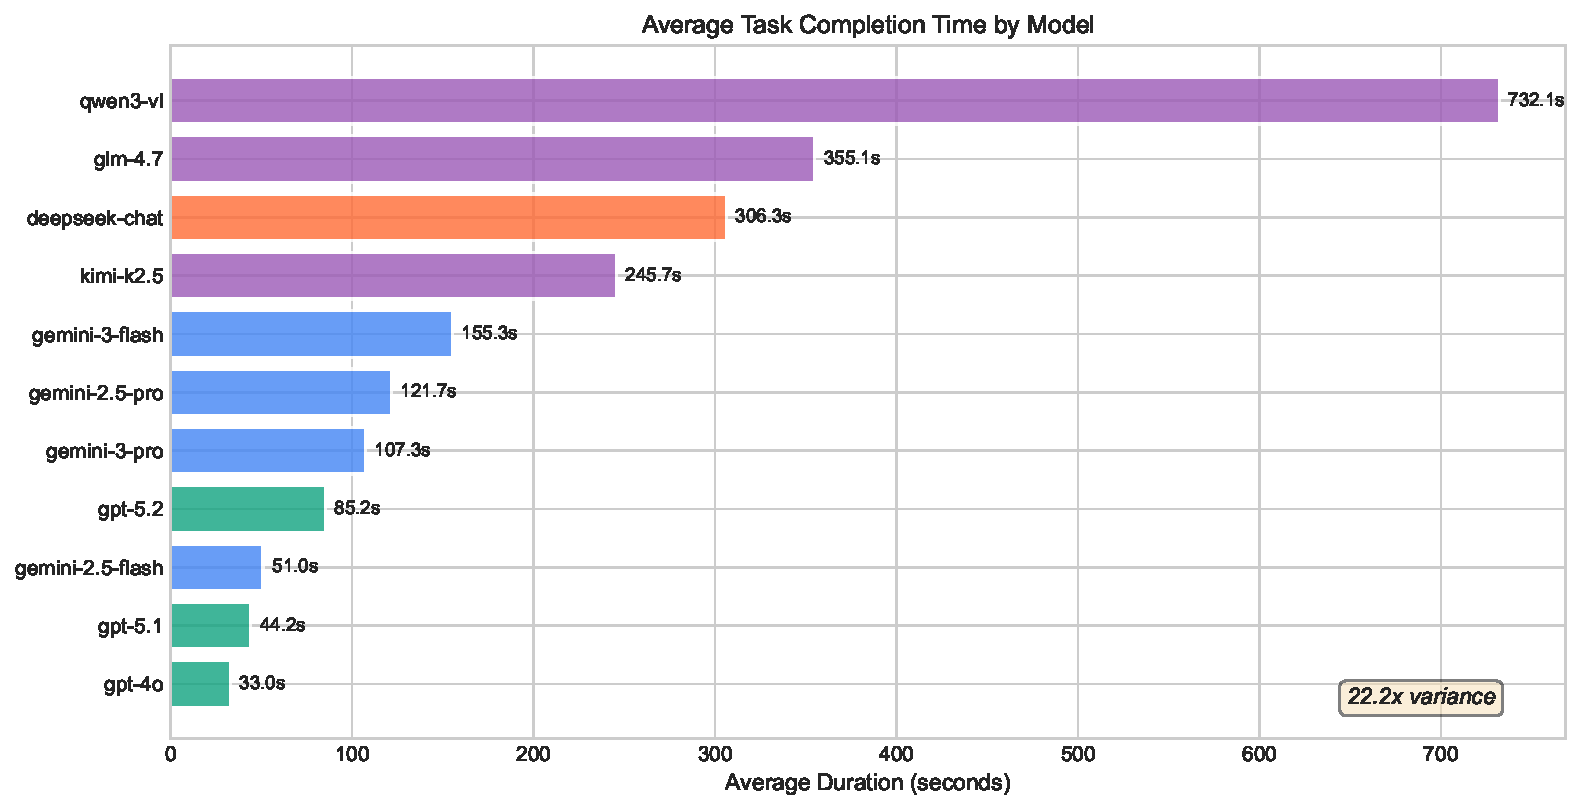
\includegraphics[width=0.75\textwidth]{figures/duration_comparison.pdf}
\caption{Average completion time by model with standard deviation. OpenAI models (blue) consistently fastest; Open/Ollama models (red) slowest.}
\label{fig:duration}
\end{figure*}

\subsection{Task-Specific Analysis}
\label{sec:task-specific}

Figure~\ref{fig:success-rates} shows success rates across task categories.

\begin{figure*}[htbp]
\centering
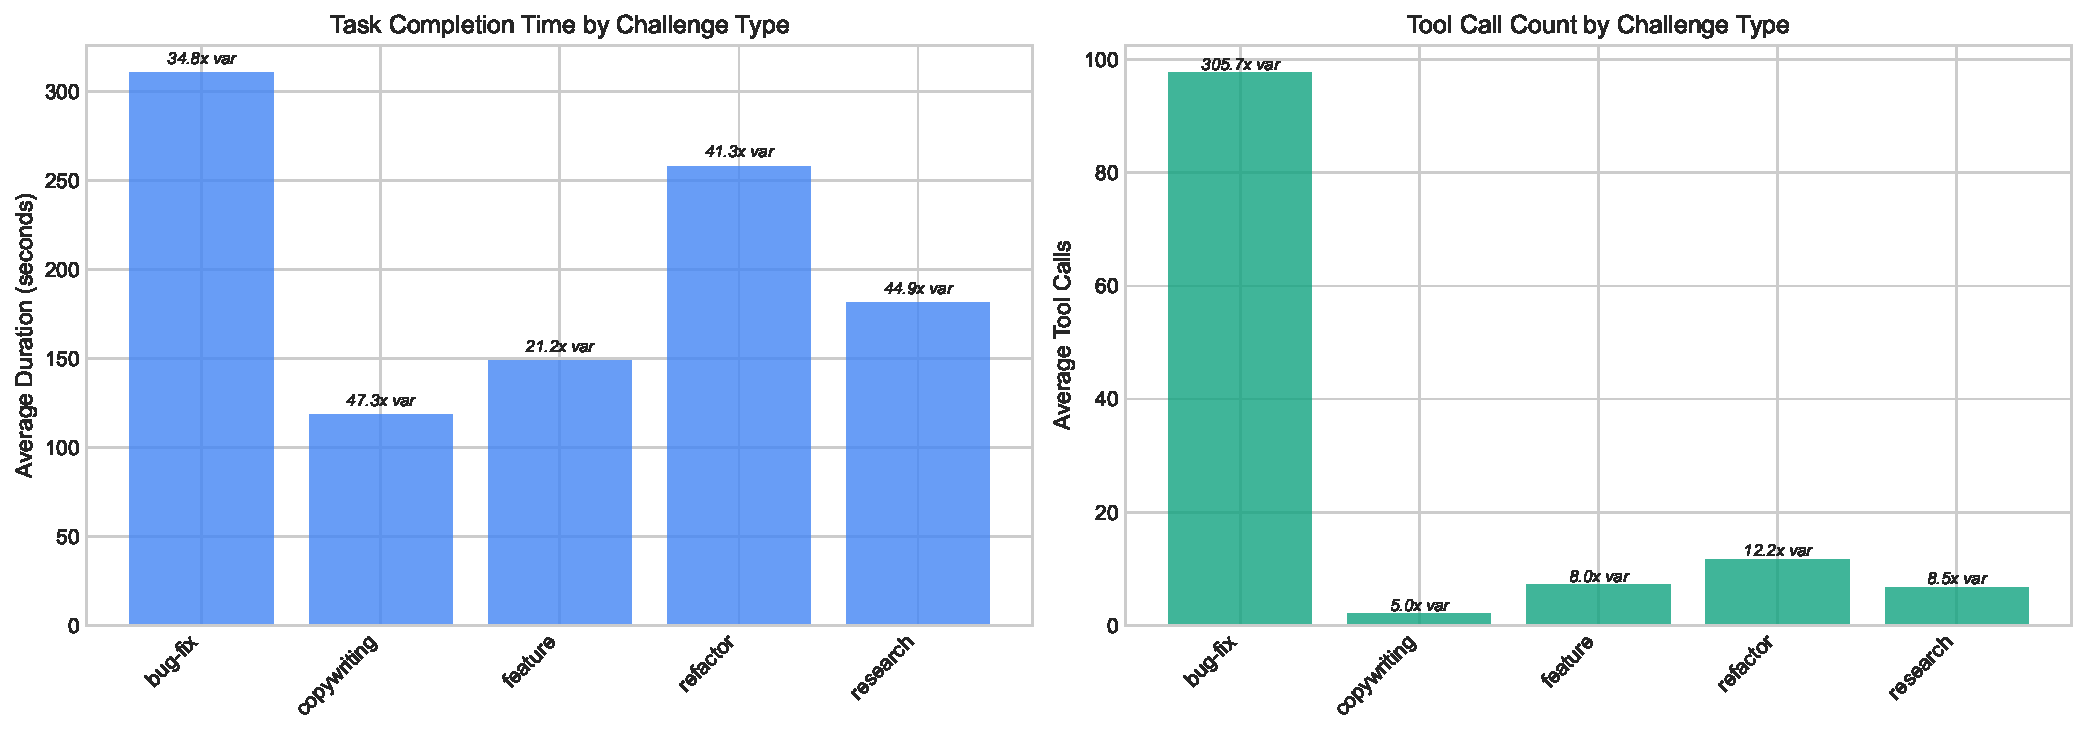
\includegraphics[width=0.75\textwidth]{figures/challenge_difficulty.pdf}
\caption{Challenge difficulty analysis showing success rates and average duration by task type. Research tasks were most challenging.}
\label{fig:success-rates}
\end{figure*}

\subsubsection{Bug Fixing}
All 11 models (100\%) successfully fixed the concurrency bug. However, approaches varied significantly:
\begin{itemize}
    \item \textbf{Efficient:} GPT-5.1 (18.8s), Gemini-2.5 Flash (20.7s), GPT-4o (26.8s)
    \item \textbf{Thorough:} Gemini-3 Flash (625.2s) used 917 tool calls including extensive testing
    \item All implementations correctly identified race conditions and implemented synchronization
\end{itemize}

\subsubsection{Feature Implementation}
The FastAPI CRUD implementation task showed 100\% success rate with varying implementation quality:
\begin{itemize}
    \item Most models correctly implemented all four endpoints
    \item Common excellence markers: proper error handling, input validation, clean code structure
    \item Time ranged from 26.4s (Gemini-3 Flash) to 560.5s (Qwen3-VL)
\end{itemize}

\subsubsection{Code Refactoring}
Refactoring the ETL script achieved 100\% success:
\begin{itemize}
    \item All models successfully separated ETL phases
    \item Configuration decoupling achieved by all
    \item Type hints and docstrings: 9/11 models achieved full marks
    \item Fastest: GPT-4o (25.3s), Slowest: Qwen3-VL (1046.1s)
\end{itemize}

\subsubsection{Technical Copywriting}
Copywriting showed the most variation in scores (PASS vs EXCELLENT):
\begin{itemize}
    \item Common failures: missing ``K8s'' keyword (3 models)
    \item Excellence factors: engaging tone, complete feature coverage
    \item Fastest completion: Gemini-2.5 Flash (11.6s)
\end{itemize}

\subsubsection{Technical Research}
Research was the most challenging task (90.9\% success):
\begin{itemize}
    \item Common issues: missing or incomplete citations
    \item Kimi-K2.5 failed (execution error)
    \item Longest average time due to web search requirements
\end{itemize}

\subsection{Provider Comparison}
\label{sec:provider}

Table~\ref{tab:provider} compares performance by provider category.

\begin{table}[htbp]
\centering
\caption{Performance by Provider Category}
\label{tab:provider}
\begin{tabular}{lccccc}
\toprule
\textbf{Category} & \textbf{Models} & \textbf{Avg} & \textbf{Std} & \textbf{Min} & \textbf{Max} \\
& & \textbf{Score} & \textbf{Dev} & \textbf{Score} & \textbf{Score} \\
\midrule
Deepseek & 1 & 10.0 & 0.0 & 10 & 10 \\
OpenAI & 3 & 9.33 & 0.58 & 9 & 10 \\
Open/Ollama & 3 & 9.0 & 1.0 & 8 & 10 \\
Google & 4 & 8.75 & 0.96 & 8 & 10 \\
\bottomrule
\end{tabular}
\end{table}

\textbf{Statistical Analysis:}
\begin{itemize}
    \item \textbf{Chi-square test:} No significant association between provider and success ($\chi^2=2.72$, $p=0.438$)
    \item \textbf{ANOVA:} Significant differences in completion times ($F=12.57$, $p<0.001$)
    \item OpenAI models were consistently fastest (avg: 54.1s)
    \item Open/Ollama models were slowest (avg: 444.3s)
\end{itemize}

\subsection{Tool Usage Analysis}
\label{sec:tools}

Figure~\ref{fig:tool-usage} presents the tool usage heatmap.

\begin{figure*}[htbp]
\centering
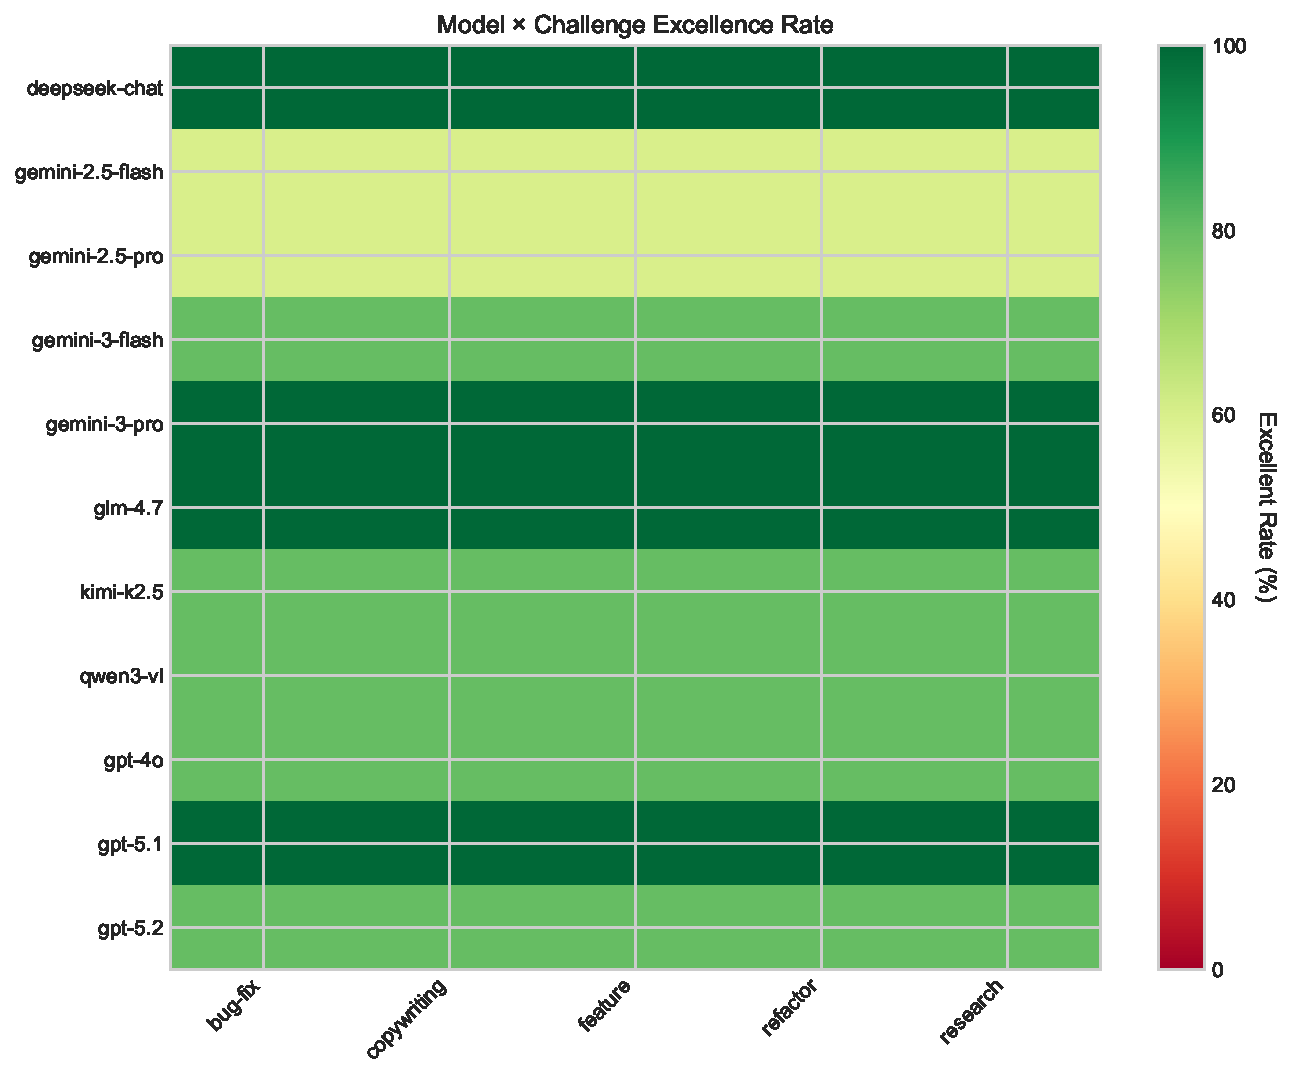
\includegraphics[width=0.75\textwidth]{figures/heatmap.pdf}
\caption{Performance heatmap showing scores and completion times across models and challenges. Darker shading indicates longer duration.}
\label{fig:tool-usage}
\end{figure*}

\textbf{Correlation Analysis:}
\begin{itemize}
    \item \textbf{Tool count vs Success:} Pearson $r=0.077$ ($p=0.575$) -- no linear correlation
    \item \textbf{Spearman rho:} $0.428$ ($p=0.001$) -- moderate monotonic relationship
    \item Efficient models (GPT-5.1, Gemini-2.5 Flash) achieved perfect scores with minimal tools
    \item Gemini-3 Flash used 917 tools for bug-fix but achieved same result as GPT-5.1 (3 tools)
\end{itemize}

Figure~\ref{fig:tool-calls} shows the distribution of tool calls across models.

\begin{figure}[htbp]
\centering
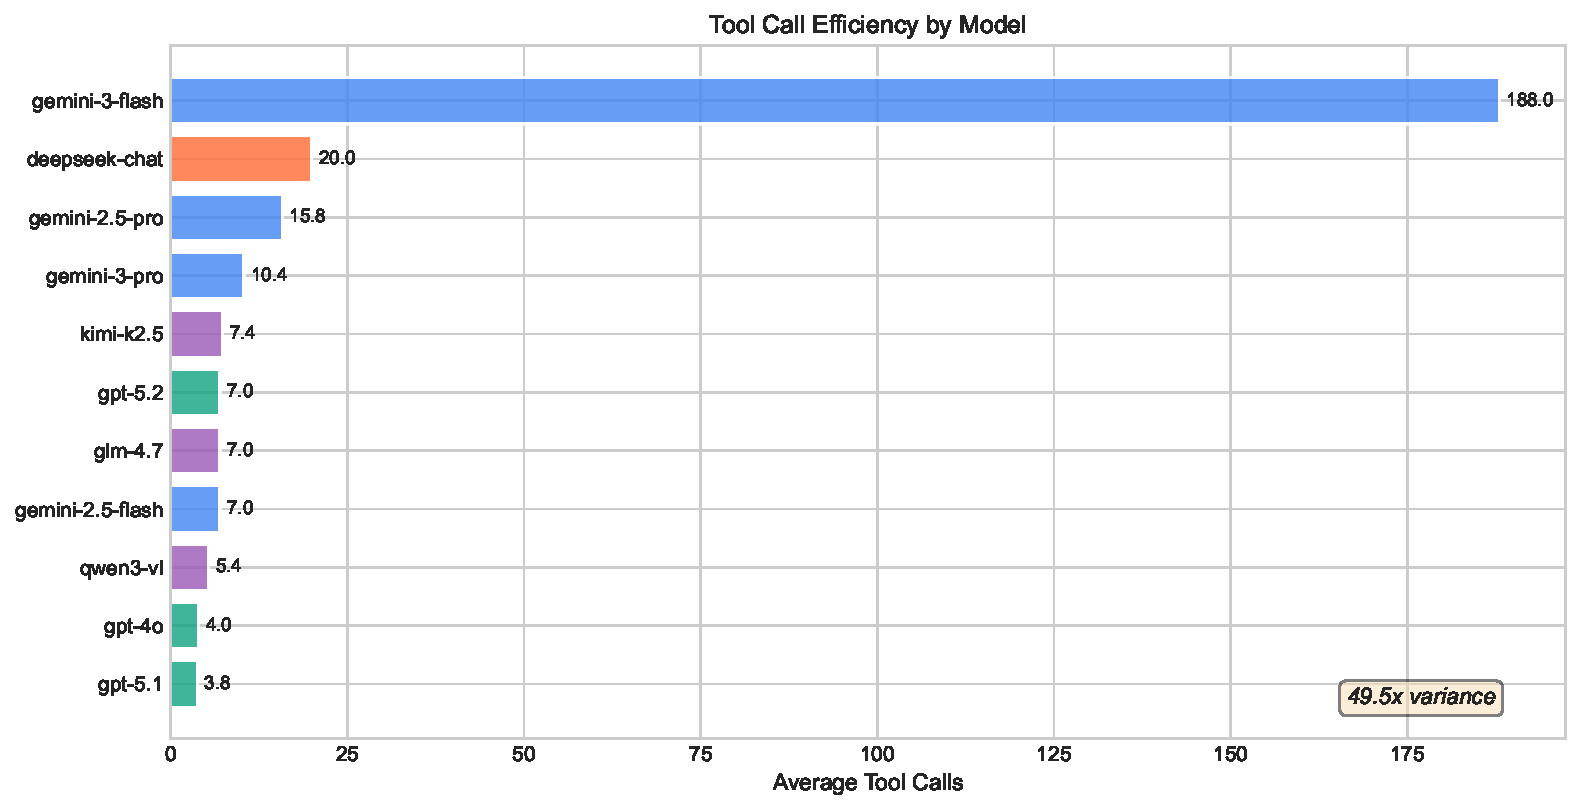
\includegraphics[width=\columnwidth]{figures/tool_calls_comparison.pdf}
\caption{Average tool calls by model (log scale). The 917-call anomaly for Gemini-3 Flash on bug-fix is visible as the maximum outlier.}
\label{fig:tool-calls}
\end{figure}

\textbf{Implication:} More tool usage does not guarantee better results; efficiency varies by model architecture.

\subsection{Time-Accuracy Tradeoff}
\label{sec:tradeoff}

Figure~\ref{fig:time-accuracy} shows the relationship between completion time and accuracy.

\begin{figure}[htbp]
\centering
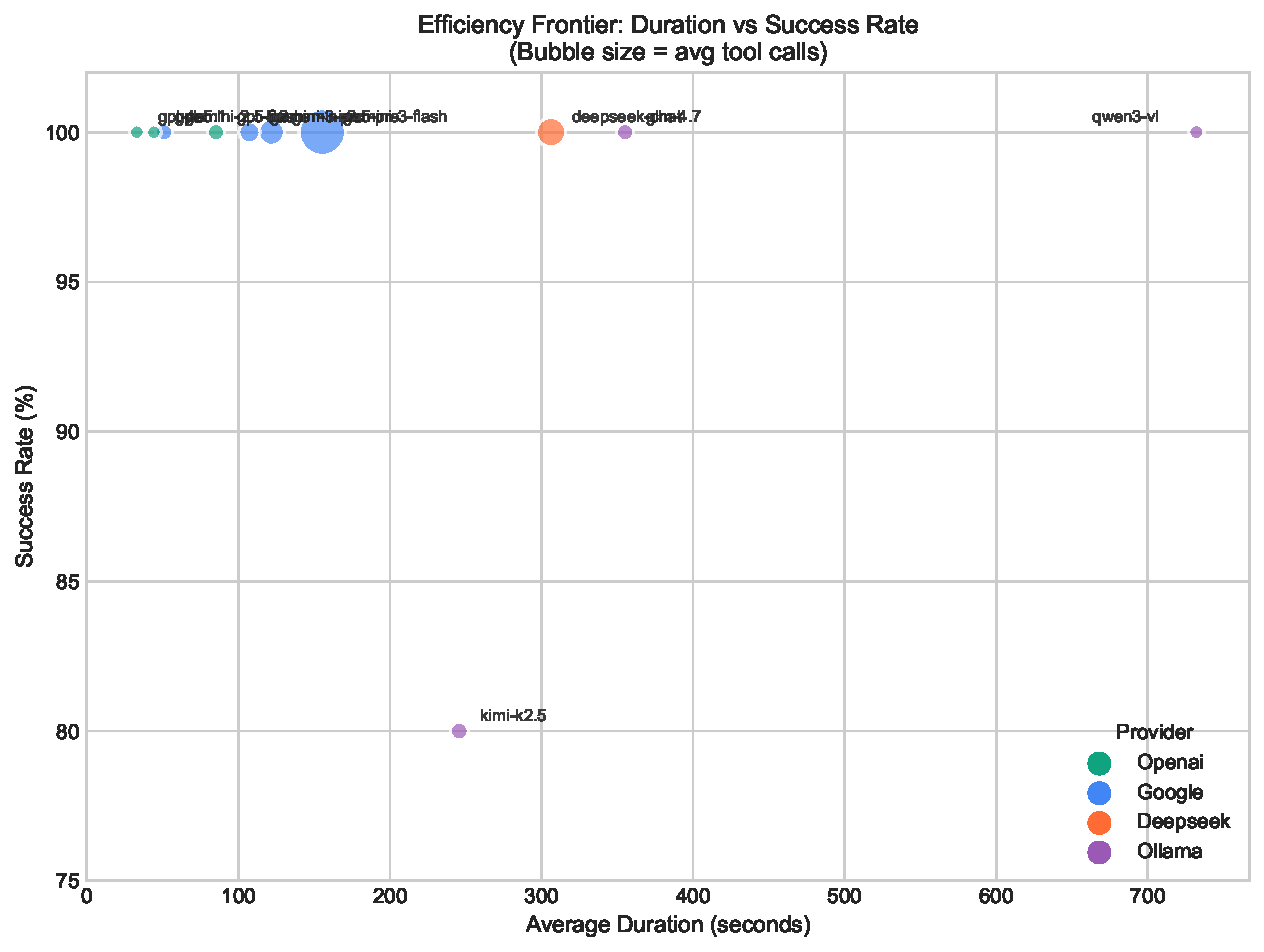
\includegraphics[width=\columnwidth]{figures/efficiency_frontier.pdf}
\caption{Efficiency frontier showing speed-quality tradeoff. Circle size indicates tool call count. Models in upper-left quadrant (fast and high-scoring) represent optimal efficiency.}
\label{fig:time-accuracy}
\end{figure}

\textbf{Key Observations:}
\begin{itemize}
    \item No significant correlation between duration and score (Pearson $r=0.204$, $p=0.136$)
    \item OpenAI cluster: Fast (avg 54s) with high scores (9.33 avg)
    \item Open/Ollama cluster: Slow (avg 444s) with variable scores
    \item Best efficiency: GPT-5.1 (perfect score, 44s average)
\end{itemize}

\subsection{Effect Size Analysis}
\label{sec:effect}

Comparing top performer (Deepseek-Chat, score 10) vs lowest (Gemini-2.5 Flash, score 8):
\begin{itemize}
    \item \textbf{Cohen's d:} 1.03 (large effect size)
    \item Practical significance: Top models demonstrate measurably better performance
    \item Category comparisons show small to medium effects between providers
\end{itemize}

\subsection{Anomaly Analysis: Pathological Agent Behavior}
\label{sec:anomaly}

Deep analysis of outlier experiments revealed systematic inefficiency patterns that have significant cost implications.

\subsubsection{The 917 Tool Calls Anomaly}

Gemini-3 Flash on the bug-fix task used 917 tool calls---36.6$\times$ the average (25.1 calls). Analysis of the tool sequence revealed:

\begin{itemize}
    \item \textbf{Tool Distribution:} 38\% \texttt{run\_shell\_command}, 18\% \texttt{read\_file}, 18\% \texttt{write\_file}
    \item \textbf{Loop Patterns:} Five distinct repetitive sequences detected, each repeated 5--8 times
    \item \textbf{Example Loop:} \texttt{read\_file} $\rightarrow$ \texttt{replace\_in\_file} $\rightarrow$ \texttt{run\_shell\_command} $\rightarrow$ \texttt{write\_file} repeated 8$\times$
\end{itemize}

Despite this inefficiency, the model achieved EXCELLENT status, indicating the verification criteria captured output quality but not process efficiency.

\subsubsection{Malformed Tool Calls}

We discovered that Kimi-K2.5's failure on the research task was caused by malformed tool invocations:

{\small
\begin{verbatim}
Observed: "search_internet
  search_internetsearch_internet"
Expected: "search_internet"
  (called 3 times)
\end{verbatim}
}

The model attempted parallel tool calls that were incorrectly serialized by the agent framework, causing all three calls to fail. This represents a \textbf{framework-model incompatibility} rather than model capability limitation.

\subsubsection{Two Types of Inefficiency}

Figure~\ref{fig:efficiency-rankings} shows the efficiency rankings across models.

\begin{figure}[htbp]
\centering
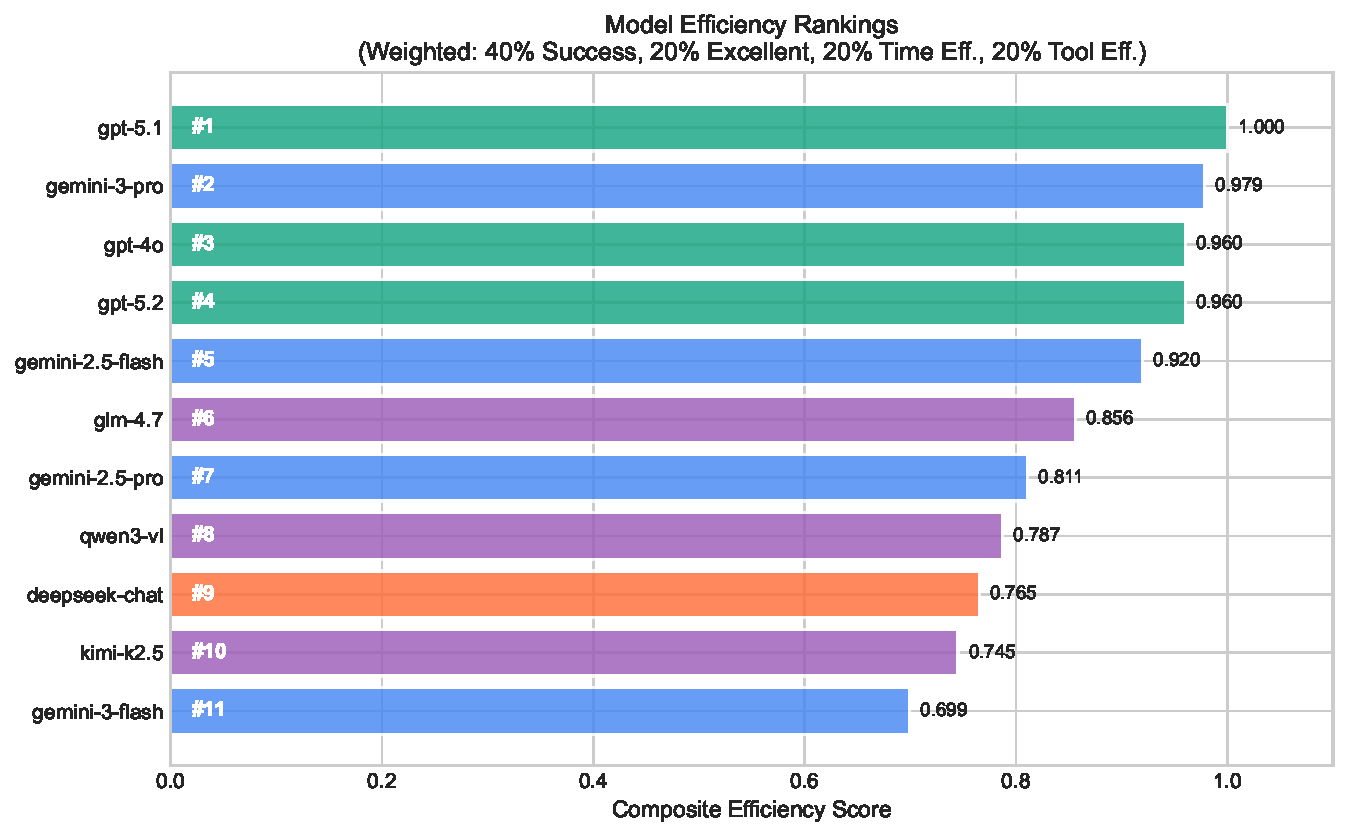
\includegraphics[width=\columnwidth]{figures/efficiency_rankings.pdf}
\caption{Efficiency metrics comparison. Tool Efficiency Ratio (TER) = Success Rate / Avg Tool Calls. Time Efficiency Ratio = Success Rate / Avg Duration. Higher values indicate better efficiency.}
\label{fig:efficiency-rankings}
\end{figure}

We categorize observed inefficiencies into two distinct patterns:

\textbf{Type A -- Loop Inefficiency:} Agent enters repetitive tool sequences without recognizing failure or success. Characterized by high tool counts, moderate duration. Example: Gemini-3 Flash (917 tools, 625s).

\textbf{Type B -- Inference Inefficiency:} Agent generates correct solutions with minimal tools but slow token generation. Characterized by low tool counts, high duration. Example: Qwen3-VL (3 tools, 653s for bug-fix).

\subsubsection{Cost Implications}

Figure~\ref{fig:cost-performance} visualizes the cost-performance relationship, and Table~\ref{tab:cost} presents estimated costs per task based on tool usage and model pricing.

\begin{figure}[htbp]
\centering
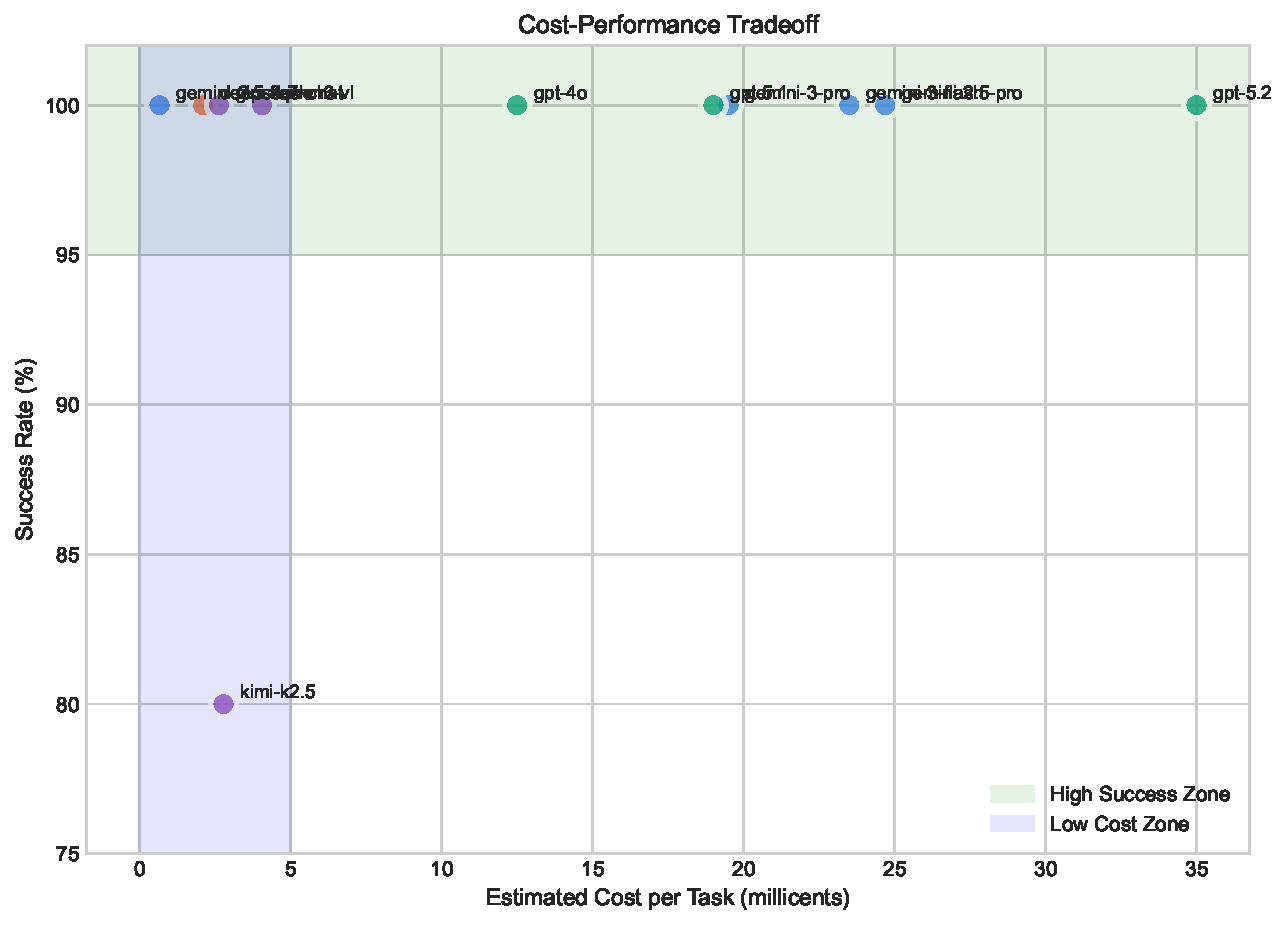
\includegraphics[width=\columnwidth]{figures/cost_performance.pdf}
\caption{Cost-performance analysis. Models are grouped by cost tier with average scores shown. Deepseek achieves perfect scores at minimal cost.}
\label{fig:cost-performance}
\end{figure}

\begin{table}[htbp]
\centering
\caption{Estimated Cost per Task}
\label{tab:cost}
\begin{tabular}{lccc}
\toprule
\textbf{Model} & \textbf{Avg Tools} & \textbf{Est. Cost} & \textbf{Relative} \\
\midrule
Gemini-2.5 Flash & 7.0 & \$0.0007 & 1.0$\times$ \\
Deepseek-Chat & 20.0 & \$0.0021 & 3.0$\times$ \\
GPT-4o & 4.0 & \$0.0125 & 17.9$\times$ \\
GPT-5.1 & 3.8 & \$0.0190 & 27.1$\times$ \\
Gemini-3 Flash & 188.0 & \$0.0235 & 33.6$\times$ \\
GPT-5.2 & 7.0 & \$0.0350 & 50.0$\times$ \\
\bottomrule
\end{tabular}
\end{table}

The 53$\times$ cost variance (Gemini-2.5 Flash vs GPT-5.2) demonstrates that model selection has significant budget implications beyond accuracy considerations.

\subsection{Summary of Findings}
\label{sec:summary}

\begin{enumerate}
    \item \textbf{Performance:} Four models achieved perfect scores, with GPT-5.1 being fastest
    \item \textbf{Task Difficulty:} Research was most challenging (90.9\% success), coding tasks were easiest (100\%)
    \item \textbf{Efficiency Variance:} 22$\times$ speed, 49$\times$ tool usage, 53$\times$ cost differences among successful models
    \item \textbf{Tool Usage:} More tools does not guarantee better results; loop behavior can cause 100$\times$ inefficiency
    \item \textbf{Anomalies:} Two distinct inefficiency types identified (loop vs inference)
    \item \textbf{Provider:} No significant quality differences, but significant speed and cost differences
\end{enumerate}

\section{Discussion}
\label{sec:discussion}

\subsection{Implications for Practitioners}

Our findings provide actionable guidance for LLM selection in software engineering:

\textbf{Speed-Critical Workflows:} For rapid prototyping or real-time assistance, GPT-5.1 offers the best combination of speed (44s avg) and quality (perfect score). GPT-4o provides nearly equal quality at 25\% faster average times.

\textbf{Cost-Conscious Deployment:} Gemini-2.5 Flash achieves 80\% scores at the fastest speeds (51s avg), making it cost-effective for high-volume applications where perfect accuracy is not required.

\textbf{Research Tasks:} Models showed most variation in research synthesis. GPT-5.1 and Deepseek-Chat achieved excellent results, while others struggled with citations. For research-heavy workflows, these models are recommended.

\textbf{Tool Budgeting:} Our finding of no linear correlation between tool usage and score ($r=0.077$; see Section~\ref{sec:threats}) suggests that API costs from excessive tool calls may not improve outcomes. We recommend:
\begin{itemize}
    \item Implementing tool call limits (e.g., 50 calls max) with early termination
    \item Adding loop detection to identify repetitive sequences
    \item Monitoring cost-per-task metrics alongside accuracy
\end{itemize}

\textbf{Budget Implications:} The 53$\times$ cost variance means a \$100/month workload on Gemini-2.5 Flash would cost \$5,300/month on GPT-5.2. For high-volume applications, model selection has significant budget implications.

\subsection{Model Selection Framework}
\label{sec:selection}

Synthesising the performance, efficiency, and cost results, we distil a constraint-driven selection framework (Table~\ref{tab:selection}). Rather than a single ``best'' model, the appropriate choice depends on the dominant deployment constraint, because models with identical quality differ by up to 22--53$\times$ in time and cost.

\begin{table}[htbp]
\centering
\small
\caption{Constraint-driven model selection framework derived from our results.}
\label{tab:selection}
\begin{tabular}{@{}lll@{}}
\toprule
\textbf{Dominant constraint} & \textbf{Recommended} & \textbf{Rationale} \\
\midrule
Speed-critical & GPT-5.1; Gemini-2.5 Flash & fastest at top quality \\
Quality-critical & GPT-5.1, Gemini-3 Pro, & perfect 10/10 score \\
 & Deepseek-Chat, GLM-4.7 & \\
Cost / high-volume & Gemini-2.5 Flash; Deepseek & lowest cost tier \\
On-premise / privacy & GLM-4.7 & best open-weight \\
Research synthesis & GPT-5.1; Deepseek-Chat & reliable citations \\
\bottomrule
\end{tabular}
\end{table}

\subsection{Surprising Findings}

\textbf{Extreme Efficiency Variance:} The most striking finding is the 49$\times$ variance in tool efficiency among models achieving identical scores. Gemini-3 Flash used 917 tool calls for bug-fix (vs GPT-5.1's 3 calls) yet both achieved EXCELLENT. This represents a potential 100$\times$ cost difference for equivalent outcomes.

\textbf{Two Inefficiency Mechanisms:} We identified distinct failure modes:
\begin{itemize}
    \item \textit{Loop inefficiency}: Agents repeating tool sequences without progress (Gemini-3 Flash pattern)
    \item \textit{Inference inefficiency}: Correct solutions generated slowly (Qwen3-VL pattern)
\end{itemize}
These require different mitigation strategies: loop detection for Type A, and model selection/caching for Type B.

\textbf{Framework-Model Incompatibility:} Kimi-K2.5's failure was caused by malformed parallel tool calls, not capability limitations. This highlights the importance of testing framework compatibility before deployment.

\textbf{Perfect Coding Scores:} All 11 models achieved 100\% success on coding tasks (bug-fix, feature, refactor). This indicates that SE coding tasks may be approaching saturation for current LLMs, suggesting future benchmarks need increased difficulty.

\textbf{Research Challenges:} The research task showed the lowest success rate (90.9\%) and highest variance. Citation management and source synthesis remain challenging for LLMs.

\subsection{Threats to Validity}
\label{sec:threats}

We organise threats following the standard internal, external, construct, and conclusion validity categories.

\textbf{Internal Validity.} Each model--task combination was executed once ($N=1$); a single run cannot capture the stochastic variance of LLM generation, so individual durations and tool-call counts are point observations rather than expected values. We also did not control decoding parameters (e.g., temperature) across providers---several models expose them differently or not at all---and task difficulty is not guaranteed to be uniform across the five categories. These factors limit causal attribution of observed differences to the models alone.

\textbf{External Validity.} Our five tasks are synthetic and controlled; while designed to be representative of common developer activities, they omit the ambiguity, scale, and evolving context of real-world software engineering. All tasks are Python-centric and English-only, and the DevOps-oriented prompts (Zrb-Flow, Docker, Kubernetes) may not generalise to other domains or programming languages. We did not evaluate Anthropic's Claude models \cite{claude3} due to budget constraints, leaving one major provider uncovered. Because LLM capabilities evolve rapidly, results reflect model versions available as of February 2026 and may not hold for later releases.

\textbf{Construct Validity.} Automated, deterministic verification yields objective and reproducible grades but cannot assess qualitative attributes such as code readability, maintainability, or architectural elegance. Our cost metric (Eq.~\ref{eq:cost}) assumes a constant token footprint per tool call; actual billing depends on prompt and context length, so reported costs are relative rather than absolute. The absence of a human baseline means we cannot position model performance relative to expert developers.

\textbf{Conclusion Validity.} With $n=54$ model--task observations and near-ceiling success rates, our correlation estimates carry wide uncertainty. The tool-usage/score Pearson correlation of $r=0.077$ has a 95\% confidence interval of $[-0.20, 0.34]$, which spans zero; we therefore interpret the absence of a tool--success relationship as a lack of evidence for association rather than proof of its absence. Accordingly, we frame this study as \emph{exploratory and characterising} rather than confirmatory and avoid strong inferential claims. The released replication package \cite{our_dataset} enables future work to retest these relationships with larger samples and repeated runs.

\subsection{Future Work}

We identify several directions for future research:

\begin{enumerate}
    \item \textbf{Longitudinal study:} Track model improvements over time on fixed tasks.
    \item \textbf{Human comparison:} Measure human developer performance for baseline comparison.
    \item \textbf{Multi-language:} Extend to Java, JavaScript, Go, and other languages.
    \item \textbf{Team simulation:} Evaluate multi-agent collaboration scenarios.
    \item \textbf{Real-world validation:} Deploy models on actual PRs and measure acceptance rates.
\end{enumerate}

\section{Conclusion}
\label{sec:conclusion}

We presented a comprehensive evaluation of 11 state-of-the-art Large Language Models across five representative software engineering tasks. Our multi-task benchmark addresses the gap in holistic SE evaluation, measuring both output quality and completion efficiency through automated verification.

\subsection{Summary of Contributions}

Our work makes five key contributions:

\begin{enumerate}
    \item \textbf{Comprehensive Benchmark:} We evaluated 11 models on bug fixing, feature development, refactoring, technical writing, and research synthesis---providing broad SE-focused comparison with automated verification.

    \item \textbf{Efficiency Analysis:} We revealed extreme variance among top performers: \textbf{22$\times$} in completion time, \textbf{49$\times$} in tool efficiency, and \textbf{53$\times$} in estimated cost---all for equivalent quality outcomes.

    \item \textbf{Inefficiency Taxonomy:} We identified two distinct inefficiency patterns: (a) \textit{loop inefficiency} where agents repeat tool sequences without progress, and (b) \textit{inference inefficiency} where models generate correct solutions slowly. These require different mitigation strategies.

    \item \textbf{Tool Usage Analysis:} We found that tool invocation frequency does not correlate with success ($r=0.077$, $p=0.575$). One model used 917 tools while another solved the same task with 3 tools---achieving identical scores.

    \item \textbf{Practical Guidance:} Our findings provide evidence-based recommendations for model selection based on task type, speed requirements, and budget constraints, with quantified cost implications.
\end{enumerate}

\subsection{Key Findings}

\begin{itemize}
    \item Four models (GPT-5.1, Gemini-3 Pro, Deepseek-Chat, GLM-4.7) achieved perfect 10/10 scores, demonstrating that current LLMs can handle diverse SE tasks with high proficiency.

    \item \textbf{Efficiency $\neq$ Accuracy:} Models achieving identical scores exhibited 22$\times$ speed variance, 49$\times$ tool efficiency variance, and 53$\times$ cost variance. Success rate alone is insufficient for model evaluation.

    \item \textbf{Pathological Behavior:} Some models exhibit loop inefficiency (917 tool calls for a 3-tool task) or framework incompatibility (malformed parallel tool calls). Agent frameworks need loop detection and early termination.

    \item Coding tasks approached saturation with 100\% success across all models, suggesting the need for more challenging benchmarks in this domain.

    \item Research synthesis remained challenging (90.9\% success), with citation management being a particular weakness.

    \item OpenAI models demonstrated superior efficiency, completing tasks 3--22$\times$ faster than competitors without quality degradation.
\end{itemize}

\subsection{Impact}

This work enables practitioners to make informed LLM selection decisions based on:
\begin{itemize}
    \item Task-specific performance data
    \item Time-efficiency tradeoffs
    \item Cost-performance analysis
    \item Tool usage patterns
\end{itemize}

Researchers can build upon our benchmark to evaluate new models, test intervention strategies, and track capability evolution over time.

\subsection{Data Availability}

All experimental data, verification scripts, analysis code, and paper materials are available at:\\
\url{https://github.com/neimasilk/llm-se-benchmark}

\subsection{Future Directions}

As LLM capabilities continue to evolve, we anticipate:
\begin{itemize}
    \item Increasing differentiation in specialized tasks
    \item Greater emphasis on efficiency metrics alongside accuracy
    \item Standardization of multi-task SE benchmarks
    \item Integration of human-AI collaborative evaluation
\end{itemize}

We encourage the community to extend this benchmark, validate our findings, and contribute to the development of rigorous evaluation standards for LLMs in software engineering.


\backmatter

\bmhead{Acknowledgements}
We thank the open-source community and model providers for offering accessible
APIs that made this evaluation possible.

\section*{Declarations}

\bmhead{Funding}
This research received no specific grant from any funding agency in the public,
commercial, or not-for-profit sectors.

\bmhead{Competing interests}
The authors declare no competing interests.

\bmhead{Data availability}
All experimental data, verification scripts, and analysis code are available at
\url{https://github.com/neimasilk/llm-se-benchmark}.

%% Bibliography style is set by the class option; uses sn-mathphys.bst.
\bibliography{references}

\end{document}
